\documentclass{beamer} 
\usetheme{default}
\usecolortheme{albatross}
\setbeamercovered{transparent}
%\usetheme{default} 
%\useoutertheme{umbcfootline} 
%\setbeamertemplate{background canvas}[vertical shading][bottom=red!20,top=yellow!30] 

\usepackage[utf8x]{inputenc}
\usepackage[spanish]{babel}
%\usepackage{beamerthemeshadow}
%\beamersetuncovermixins{\opaqueness<1>{25}}{\opaqueness<2->{15}}

%\usepackage{lmodern}
% elimina las siguientes advertencias:
% LaTeX Font Warning: Font shape `OT1/cmss/m/n' in size <4> not available
% (Font)              size <5> substituted on input line 22.
% LaTeX Font Warning: Size substitutions with differences
% (Font)              up to 1.0pt have occurred.
%

% cuando  \titel{} \author{} posiciona despues \begin{document} ,
% aparece eso  advertencia: :
% Package hyperref Warning: Option `pdfauthor' has already been used,
% (hyperref) ... 
% Por tanto posiciona lo antes de  \begin{document}

\title{Introducción a la programación}   
\author{Manuel J. Molino \and Luis Molina}
\institute{IES Virgen del Carmen \and Departamento de informatica}
\date{\today} 


% Adicional intercala package{beamerthemeshadow} 
%  causa que elementos que aparece en el futuro 
%  escribe ligero 
% funciona por tablas tambien cuando aplica teTeX
\begin{document}


\begin{frame}
\titlepage %portada
\end{frame} 

\begin{frame}
\frametitle{Índice}
\tableofcontents
\end{frame} 


\section{Arquitectura Von Neumann}
\begin{frame}
\begin{center}
\begin{Huge}
ARQUITECTURA\\DE LA\\\vspace{0.7cm} COMPUTADORA
\end{Huge}
\end{center}
\end{frame} 

\begin{frame}
\frametitle{Arquitectura Von Neumann} 
\begin{figure}
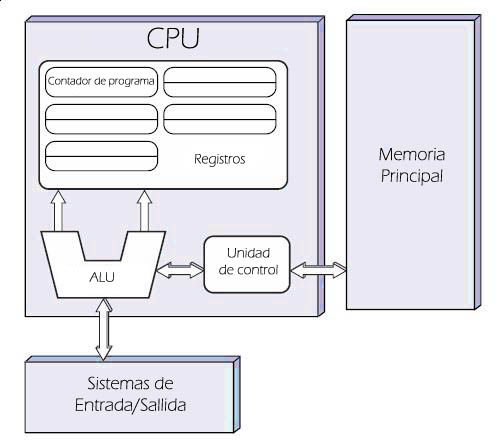
\includegraphics[scale=0.35]{imagenes/Arquitecturaneumann.jpg} 
\caption{Arquitectura Von Neumann}
\end{figure} 
\end{frame}

\begin{frame}
\frametitle{Arquitectura Von Neumann}
\begin{itemize}[<+->]
\item Obten la siguiente instrucción desde la memoria en la dirección indicada por el contador de programa y la guarda en el registro de instrucción.
\item Aumenta el contador de programa en la longitud de la instrucción para apuntar a la siguiente.
\item Descodifica la instrucción mediante la unidad de control. Ésta se encarga de coordinar el resto de componentes del ordenador para realizar una función determinada.
\item Ejecuta la instrucción. Ésta puede cambiar el valor del contador del programa, permitiendo así operaciones repetitivas.
\item Regresa al paso 1
\end{itemize} 
\end{frame}

\begin{frame}
\frametitle{Esquema de una computadora} 
\begin{figure}
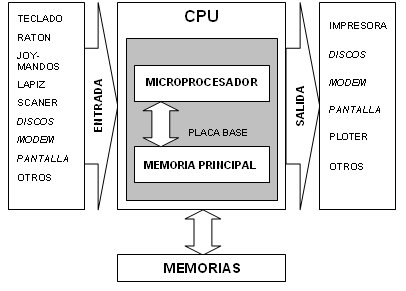
\includegraphics[scale=0.7]{imagenes/esquemaOrdenador.jpg} 
\caption{Computadora}
\end{figure} 
\end{frame}

\begin{frame}
\frametitle{Interior de una computadora} 
\begin{figure}
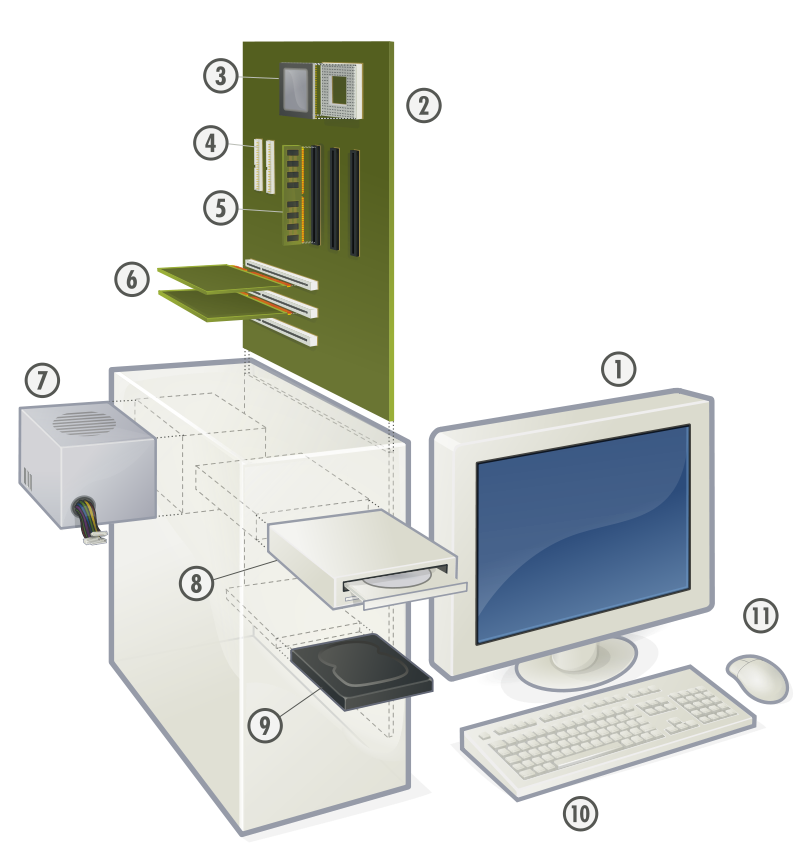
\includegraphics[scale=0.25]{imagenes/ordenador.png} 
\caption{Computadora}
\end{figure} 
\end{frame}

\begin{frame}
\frametitle{Interior de una computadora} 
\begin{figure}
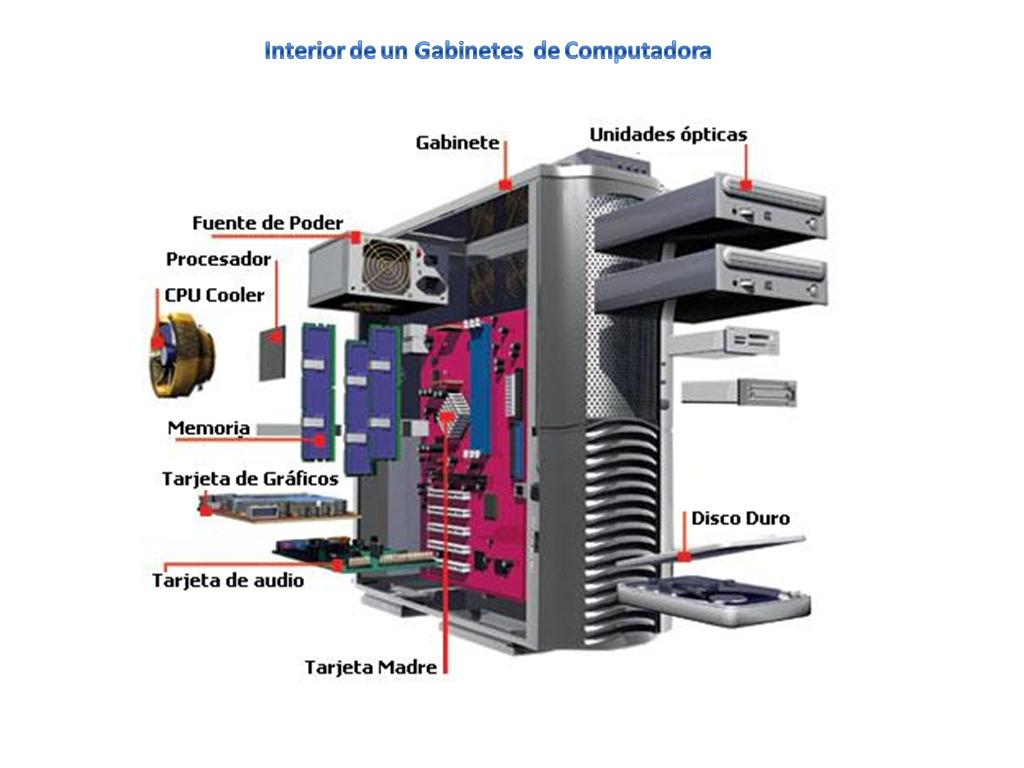
\includegraphics[scale=0.35]{imagenes/ordenador.jpg} 
\caption{Computadora}
\end{figure} 
\end{frame}

\begin{frame} 
\frametitle{Componentes del computador}
\begin{itemize}[<+->]
\item CPU.
\item Unidad de memoria.
\item Dispositivos de almacenamiento (discos, cintas, CDs, \dots)
\item Dispositivos de I/O (monitor, teclado, impresora, \dots).
\item Dispositivos de comunicación (modem, tarjetas de red, \dots).
\end{itemize} 
\end{frame}


\section{Arranque del computador}

\begin{frame} 
\frametitle{Arranque del computador}
\begin{itemize}[<+->]
\item \alert{BIOS} Chequea el funcionamiento de los dispositivos de la computadoras.
\item \alert{booting} secuencia de instrucciones de inicialización o de arranque del ordenador (\emph{CMOS})
\item \alert{boot sector} generalmente el primer sector del disco duro (\emph{MBR}) contiene las instrucciones necesarias que permiten realizar el proceso de carga en la memoria RAM de una parte de los ficheros del sistema operativo que se encuentra grabado en la partición activa del disco duro y que permite iniciar el proceso de carga.
\item \alert{Windows XP} el fichero que asume la función de cargador del sistema se denomina \emph{NTLDRE}
\item \alert{GRUB} carga el sistema operativo y le transferir el control (\emph{GNU/Linux})
\end{itemize} 
\end{frame}

\begin{frame}[fragile]
\frametitle{UEFI}
\begin{itemize}[<+->]
\item \textbf{Interfaz Extensible del Firmware, Extensible Firmware Interface (EFI).}
\item Es una especificación desarrollada por Intel dirigida a reemplazar la antigua interfaz del estándar IBM PC ROM BIOS.
\item Interactúa como puente entre el sistema operativo y el firmware base.
\end{itemize}
\end{frame}

\section{Kernel} 

\begin{frame}
\frametitle{Núcleo del sistema operativo}
Cuando arrancas un ordenador con cualquier sistema operativo, el Kernel se carga en memoria y permanece allí hasta que apagas el equipo, realizando funciones básicas como pueden ser:\pause
\begin{itemize}[<+->]
\item Comunicación entre procesos.
\item Control de periféricos
\item Manejo de memoria.
\item Control de interrupciones.
\end{itemize} 
\end{frame}

\begin{frame}
\frametitle{Kernel} 
\begin{figure}
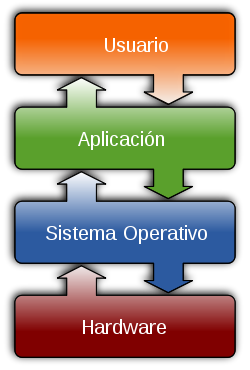
\includegraphics[scale=0.35]{imagenes/kernel.png} 
\caption{Gestión del sistema operativo}
\end{figure} 
\end{frame}

\section{Memoria}
\begin{frame}
\frametitle{Gestión de memoria}
\begin{itemize}[<+->]
\item La administración de memoria es el corazón de los sistemas operativos. 
\item Es importante en la administración del sistema como en \emph{programación}
\item Cada proceso en un sistema operativo multitarea se ejecuta en espacio de memoria. (\emph{sandbox})
\item Este sandbox es el espacio virtual de direcciones.
\item  Estas direcciones virtuales son mapeadas a direcciones físicas mediante tablas de páginas, mantenidas estas por el kernel del sistema operativo y consultadas por el procesador. 
\item Tenemos dos espacios de memoria \emph{el del kernel y el de usuario} 
\item Una porción del espacio de direcciones virtuales deberá ser reservado para el kernel. 
\item Cada proceso tiene su propio set de tablas de páginas.
\end{itemize} 
\end{frame}

\begin{frame}
\frametitle{Memoria} 
\begin{figure}
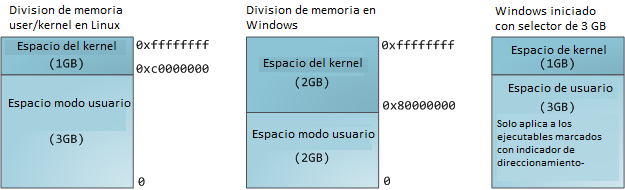
\includegraphics[scale=0.65]{imagenes/memoria1.png} 
\caption{Espacio de memoria}
\end{figure} 
\end{frame}

\begin{frame}
\frametitle{Memoria} 
\begin{figure}
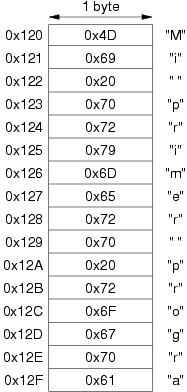
\includegraphics[scale=0.5]{imagenes/stringstore.png}
\caption{Almacenamiento de un string}
\end{figure} 
\end{frame}

\begin{frame}
\frametitle{Memoria de un proceso}
En el caso de un programa en C para Unix y para casi todos los otros sistemas operativos, cada proceso se organizar en cuatro áreas de memoria, que se llaman segmentos:\pause
\begin{description}[<+->]
\item[Segmento de código] Es donde se encuentra el código ejecutable del programa. 
\item[Segmento de datos] Es donde se encuentran las variables globales y las variables declaradas como estáticas,
\item[El montón o heap]  Es la zona donde se almacena la memoria reservada dinámicamente.  
\item[La pila o stack] Funciona como una pila (\emph{LIFO})   
\end{description} 
\end{frame}

\begin{frame}
\frametitle{Memoria} 
\begin{figure}
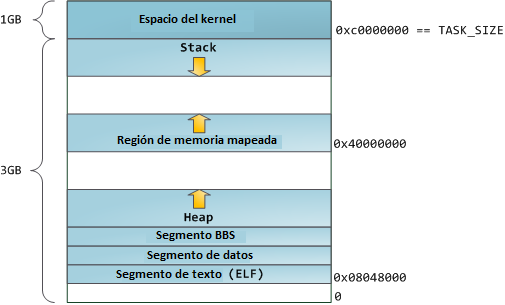
\includegraphics[scale=0.65]{imagenes/memoria2.png} 
\caption{Espacio de memoria}
\end{figure} 
\end{frame}

\begin{frame}
\begin{center}
\begin{Huge}
LENGUAJES DE \\\vspace{0.7cm} PROGRAMACIÓN
\end{Huge}
\end{center}
\end{frame} 

\section{Historia lenguajes de programación} 

\begin{frame}
\frametitle{Lenguajes} 
\begin{figure}
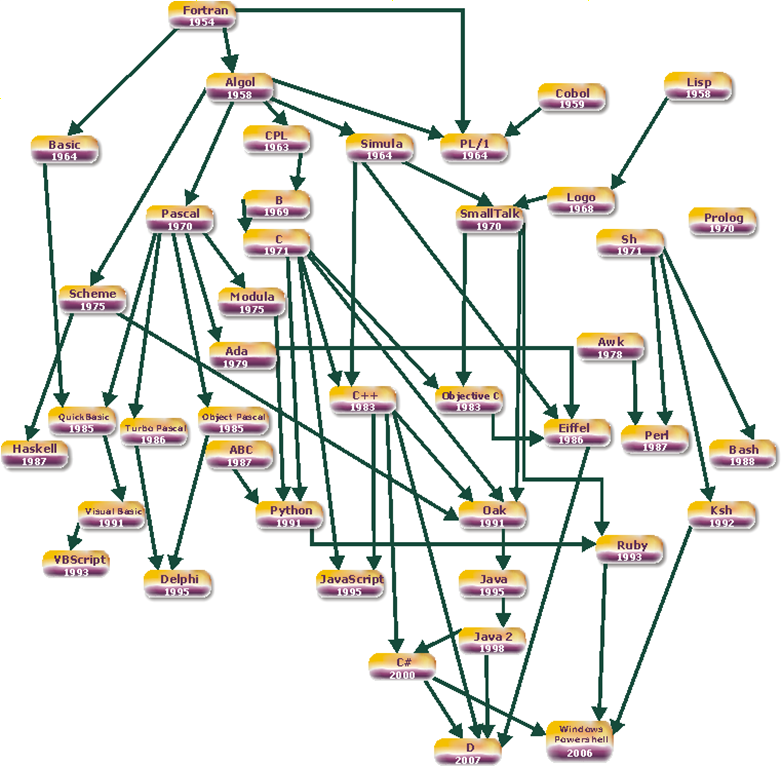
\includegraphics[scale=0.28]{imagenes/histprog1.png} 
\caption{Evolución de los lenguajes de programación}
\end{figure} 
\end{frame}

\begin{frame}
\frametitle{Clasificación de los lenguajes de programación}
\begin{block}{Proximidad máquina}
\begin{itemize}
\item Primera generación.
\item Segunda generación.
\item Tercera generación.
\item Cuarta generación.
\end{itemize}
\end{block}
\pause
\begin{block}{Forma de ejecutarse}
\begin{itemize}
\item Lenguajes compilados.
\item Lenguajes interpretados.
\end{itemize}
\end{block}
\end{frame}

\begin{frame}
\frametitle{Lenguajes primera generación}
\framesubtitle{Código máquina}
\begin{enumerate}[<+->]
\item El lenguaje de máquina o código máquina es el sistema de códigos directamente interpretable por un circuito microprogramable, como el microprocesador de una computadora o el microcontrolador de un autómata. 
\item Este lenguaje está compuesto por un conjunto de instrucciones que determinan acciones al ser tomadas por la máquina.  
\item Un programa consiste en una cadena de estas instrucciones más un conjunto de datos sobre el cual se trabaja. 
\item Tanto los datos como las intrucciones son un \emph{chorro} de 0 y 1
\end{enumerate}
\end{frame}

\begin{frame}
\frametitle{Código máquina} 
\begin{figure}
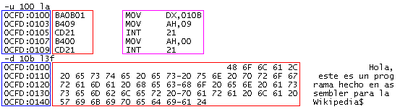
\includegraphics[scale=0.9]{imagenes/codmaq.png} 
\caption{Lenguaje máquina}
\end{figure} 
\end{frame}

\begin{frame}
\frametitle{Lenguajes segunda generación}
\framesubtitle{Lenguaje ensamblador}
\begin{enumerate}[<+->]
\item Implementa una representación simbólica de los códigos de máquina binarios.  
\item basada en los mnemónicos que simbolizan las instrucciones, los registros del procesador, las posiciones de memoria y otras características del lenguaje. 
\item Un lenguaje ensamblador es por lo tanto específico de cierta arquitectura de computador física 
\item Muchos dispositivos programables (como los microcontroladores) aún cuentan con el ensamblador como la única manera de ser manipulados. 
\end{enumerate}
\end{frame}

\begin{frame}[fragile]
\frametitle{Ensamblador} 
\begin{tiny}
\begin{verbatim}
; ---------------------------------------------
; Programa que imprime un string en la pantalla
; ---------------------------------------------
        .model small               ; modelo de memoria
        .stack                     ; segmento del stack
        .data                      ; segmento de datos
        Cadena1 DB 'Hola Mundo.$'  ; string a imprimir (finalizado en $)
        .code                      ; segmento del código
 
; ---------------------------------------------
; Inicio del programa
; ---------------------------------------------
        programa:
                MOV AX, @data           ; carga en AX la dirección del segmento de datos
                MOV DS, AX              ; mueve la dirección al registro de segmento por medio de AX
                MOV DX, offset Cadena1  ; mueve a DX la dirección del string a imprimir
                MOV AH, 9               ; AH = código de la función del MS DOS para imprimir un string en la pantalla
                INT 21h                 ; llamada al MS DOS para imprimir un string en la pantalla
                INT 20h                 ; llamada al MS DOS para finalizar el programa
        end programa
\end{verbatim} 
\end{tiny}
\end{frame}


\begin{frame}
\frametitle{Lenguajes tercera generación}
\begin{itemize}[<+->]
\item El código vale para cualquier máquina pero deberá ser traducido mediante software especial que adaptará el código de alto nivel al código máquina correspondiente.  
\item Ejemplos:
\begin{enumerate}
\item Fortran.
\item Cobol.
\item Basic.
\item Algol.
\item C.
\item Pascal.
\item Lisp
\item Smalltalk.
\item Prolog
\end{enumerate}
\end{itemize}
\end{frame}

\begin{frame}[fragile]
\frametitle{Lenguajes tercera generación} 
\begin{block}{Pascal}
\begin{verbatim}
PROGRAM HOLA
 PRINT *, '¡Hola, mundo!'
END
\end{verbatim}
\end{block}
\pause
\begin{exampleblock}{Lisp}
\begin{verbatim}
(format t "¡Hola, mundo!")
\end{verbatim}
\end{exampleblock}
\pause
\begin{alertblock}{C}
\begin{verbatim}
#include <stdio.h>
int main(){
        printf("Hola mundo");
        return 0; }
\end{verbatim}
\end{alertblock}
\end{frame}

\begin{frame}
\frametitle{Lenguajes cuarta generación}
\begin{itemize}[<+->]
\item Con ciertas herramientas prefabricadas, que aparentemente dan lugar a un lenguaje de programación de alto nivel.
\item Algunos restringen el nombre de lenguajes de cuarta generación para los lenguajes orientados a objetos.
\item Ejemplos:
\begin{enumerate}
\item NATURAL.
\item PL/SQL.
\item ...
\end{enumerate}
\end{itemize}
\end{frame}

\section{Clasificación de los lenguajes de programación}

\begin{frame}
\frametitle{Lenguajes compilados}
Un lenguaje compilado es una expresión un tanto imprecisa para referirse a un lenguaje de programación que se implementa mediante un compilador.
\pause
\begin{itemize}[<+->]
\item Un compilador es un programa informático que traduce un programa escrito en un lenguaje de programación a otro lenguaje de programación.
\item Usualmente el segundo lenguaje es lenguaje de máquina, pero también puede ser un código intermedio (bytecode).
\item Ejemplo:
\begin{enumerate}
\item Pascal.
\item C.
\item Fortran.
\item Ada.
\end{enumerate}
\end{itemize}
\end{frame}

\begin{frame}
\frametitle{Lenguajes interpretados}
Un lenguaje interpretado es un lenguaje de programación que está diseñado para ser ejecutado por medio de un intérprete, en contraste con los lenguajes compilados.
\pause
\begin{itemize}[<+->]
\item Independencia de plataforma (por ejemplo el byte code de Java).
\item Programas de tamaño pequeño.
\item Usualmente son mucho menos eficiente que la ejecución de un programa compilado.
\item Ejemplo:
\begin{enumerate}
\item Perl.
\item Python.
\item Ruby.
\item PHP.
\item Javascript.
\item Visual Basic.
\end{enumerate}
\end{itemize}
\end{frame}

\begin{frame}
\frametitle{Java}
\begin{small}
\begin{itemize}[<+->]
\item Las aplicaciones de Java son generalmente compiladas a bytecode (clase Java).
\item Puede correr en cualquier máquina virtual Java (JVM) sin importar la arquitectura de la computadora.
\item Usa el paradigma de la programación orientada a objetos.
\item Permite la ejecución de un mismo programa en múltiples sistemas operativos.
\item El axioma de Java, \emph{write once, run anywhere}
\item \alert{Bytecodes} instrucciones máquina simplificadas específicas de la plataforma Java.
\item El \emph{bytecode} está a medio camino entre el código fuente y el código máquina .
\item El bytecode es ejecutado entonces en la máquina virtual (JVM), un programa escrito en código nativo de la plataforma destino (que es el que entiende su hardware), que interpreta y ejecuta el código.
\item ¿JVM es dependiente del Sistema Operativo?
\end{itemize}
\end{small}
\end{frame}

\begin{frame}
\frametitle{Tipos de programación}
\begin{block}{Programación estructurada}
\begin{itemize}[<+->]
\item Orientada a mejorar la claridad, calidad y tiempo de desarrollo.
\item Utiliza únicamente subrutinas y tres estructuras: secuencia, selección (if y switch) e iteración (bucles for y while).
\item Es posible hacer la programación estructurada en cualquier lenguaje de programación
\end{itemize}
\end{block}
\pause
\begin{block}{Programación orientada a objetos}
\begin{itemize}[<+->]
\item Usa los objetos en sus interacciones, para diseñar aplicaciones y programas informáticos.
\item Los objetos son entidades que tienen un determinado estado, comportamiento (método) e identidad.
\end{itemize}
\end{block}
\end{frame}

\begin{frame}
\frametitle{Lenguajes OO}
\begin{enumerate}
\item C++.
\item C\#.
\item Java.
\item Smalltalk.
\item Ruby.
\item Python.
\item Visual Basic.
\item ...
\end{enumerate}
\end{frame}

\begin{frame}[fragile]
\frametitle{Java OO}
\begin{verbatim}
public class MiPrimeraClase {
        int x;
        int y;

        MiPrimeraClase(int x, int y) {
            this.x = x;
            this.y = Y;
        }

        int getX() {
                return x;
        }

        void setX(int x) {
                this.x = x;
        }
        ....................
}
\end{verbatim}
\end{frame}

\section{Programa informático} 

\begin{frame}
\frametitle{¿Qué es un programa?}
\begin{itemize}[<+->]
\item Un programa informático es un conjunto de instrucciones que una vez ejecutadas realizarán una o varias tareas en una computadora.
\item Al conjunto general de programas, se le denomina \emph{software}.
\item La programación de computadoras es el proceso iterativo de escribir o editar código fuente. 
\item Una vez escrito el código fuente:
\begin{enumerate}
\item Mediante un programa se adptan las instrucciones conforme son encontradas. A este proceso se lo llama interpretar.
\item Traduciendo el código escrito del programa a su equivalente en lenguaje máquina. A este proceso se le llama compilar y al programa traductor se le denomina compilador..
\end{enumerate}
\end{itemize}
\end{frame}

\begin{frame}
\frametitle{Programas}
\begin{itemize}[<+->]
\item Procesador texto.
\item Navegador.
\item Programas para enviar correo. 
\item \dots
\item Todo este software es desarrollado mediante lenguajes de programación.
\end{itemize}
\end{frame}


\begin{frame}
\frametitle{¿Cómo se ejecuta?}
\begin{itemize}[<+->]
\item Típicamente, los programas se almacenan en una memoria no volátil (por ejemplo un disco) para que luego el usuario de la computadora, directa o indirectamente, solicite su ejecución.
\item El programa es cargado en la memoria de acceso aleatorio o RAM del equipo, bajo el control del software llamado sistema operativo, el cual puede acceder directamente al procesador. 
\item El procesador ejecuta (corre) el programa, instrucción por instrucción hasta que termina.
\item A un programa en ejecución se le suele llamar también proceso. 
\item Un programa puede terminar su ejecución en forma normal o por causa de un error, dicho error puede ser de software o de hardware.
\end{itemize}
\end{frame}


\begin{frame}
\frametitle{Preguntas} 
\begin{figure}

\includegraphics[scale=0.9]{imagenes/dudas.png} 
\caption{Lenguaje máquina}
\end{figure} 
\end{frame}


\end{document}

